\documentclass[11pt]{article}

    \usepackage[breakable]{tcolorbox}
    \usepackage{parskip} % Stop auto-indenting (to mimic markdown behaviour)
    
    \usepackage{iftex}
    \ifPDFTeX
    	\usepackage[T1]{fontenc}
    	\usepackage{mathpazo}
    \else
    	\usepackage{fontspec}
    \fi

    % Basic figure setup, for now with no caption control since it's done
    % automatically by Pandoc (which extracts ![](path) syntax from Markdown).
    \usepackage{graphicx}
    % Maintain compatibility with old templates. Remove in nbconvert 6.0
    \let\Oldincludegraphics\includegraphics
    % Ensure that by default, figures have no caption (until we provide a
    % proper Figure object with a Caption API and a way to capture that
    % in the conversion process - todo).
    \usepackage{caption}
    \DeclareCaptionFormat{nocaption}{}
    \captionsetup{format=nocaption,aboveskip=0pt,belowskip=0pt}

    \usepackage[Export]{adjustbox} % Used to constrain images to a maximum size
    \adjustboxset{max size={0.9\linewidth}{0.9\paperheight}}
    \usepackage{float}
    \floatplacement{figure}{H} % forces figures to be placed at the correct location
    \usepackage{xcolor} % Allow colors to be defined
    \usepackage{enumerate} % Needed for markdown enumerations to work
    \usepackage{geometry} % Used to adjust the document margins
    \usepackage{amsmath} % Equations
    \usepackage{amssymb} % Equations
    \usepackage{textcomp} % defines textquotesingle
    % Hack from http://tex.stackexchange.com/a/47451/13684:
    \AtBeginDocument{%
        \def\PYZsq{\textquotesingle}% Upright quotes in Pygmentized code
    }
    \usepackage{upquote} % Upright quotes for verbatim code
    \usepackage{eurosym} % defines \euro
    \usepackage[mathletters]{ucs} % Extended unicode (utf-8) support
    \usepackage{fancyvrb} % verbatim replacement that allows latex
    \usepackage{grffile} % extends the file name processing of package graphics 
                         % to support a larger range
    \makeatletter % fix for grffile with XeLaTeX
    \def\Gread@@xetex#1{%
      \IfFileExists{"\Gin@base".bb}%
      {\Gread@eps{\Gin@base.bb}}%
      {\Gread@@xetex@aux#1}%
    }
    \makeatother

    % The hyperref package gives us a pdf with properly built
    % internal navigation ('pdf bookmarks' for the table of contents,
    % internal cross-reference links, web links for URLs, etc.)
    \usepackage{hyperref}
    % The default LaTeX title has an obnoxious amount of whitespace. By default,
    % titling removes some of it. It also provides customization options.
    \usepackage{titling}
    \usepackage{longtable} % longtable support required by pandoc >1.10
    \usepackage{booktabs}  % table support for pandoc > 1.12.2
    \usepackage[inline]{enumitem} % IRkernel/repr support (it uses the enumerate* environment)
    \usepackage[normalem]{ulem} % ulem is needed to support strikethroughs (\sout)
                                % normalem makes italics be italics, not underlines
    \usepackage{mathrsfs}
    

    
    % Colors for the hyperref package
    \definecolor{urlcolor}{rgb}{0,.145,.698}
    \definecolor{linkcolor}{rgb}{.71,0.21,0.01}
    \definecolor{citecolor}{rgb}{.12,.54,.11}

    % ANSI colors
    \definecolor{ansi-black}{HTML}{3E424D}
    \definecolor{ansi-black-intense}{HTML}{282C36}
    \definecolor{ansi-red}{HTML}{E75C58}
    \definecolor{ansi-red-intense}{HTML}{B22B31}
    \definecolor{ansi-green}{HTML}{00A250}
    \definecolor{ansi-green-intense}{HTML}{007427}
    \definecolor{ansi-yellow}{HTML}{DDB62B}
    \definecolor{ansi-yellow-intense}{HTML}{B27D12}
    \definecolor{ansi-blue}{HTML}{208FFB}
    \definecolor{ansi-blue-intense}{HTML}{0065CA}
    \definecolor{ansi-magenta}{HTML}{D160C4}
    \definecolor{ansi-magenta-intense}{HTML}{A03196}
    \definecolor{ansi-cyan}{HTML}{60C6C8}
    \definecolor{ansi-cyan-intense}{HTML}{258F8F}
    \definecolor{ansi-white}{HTML}{C5C1B4}
    \definecolor{ansi-white-intense}{HTML}{A1A6B2}
    \definecolor{ansi-default-inverse-fg}{HTML}{FFFFFF}
    \definecolor{ansi-default-inverse-bg}{HTML}{000000}

    % commands and environments needed by pandoc snippets
    % extracted from the output of `pandoc -s`
    \providecommand{\tightlist}{%
      \setlength{\itemsep}{0pt}\setlength{\parskip}{0pt}}
    \DefineVerbatimEnvironment{Highlighting}{Verbatim}{commandchars=\\\{\}}
    % Add ',fontsize=\small' for more characters per line
    \newenvironment{Shaded}{}{}
    \newcommand{\KeywordTok}[1]{\textcolor[rgb]{0.00,0.44,0.13}{\textbf{{#1}}}}
    \newcommand{\DataTypeTok}[1]{\textcolor[rgb]{0.56,0.13,0.00}{{#1}}}
    \newcommand{\DecValTok}[1]{\textcolor[rgb]{0.25,0.63,0.44}{{#1}}}
    \newcommand{\BaseNTok}[1]{\textcolor[rgb]{0.25,0.63,0.44}{{#1}}}
    \newcommand{\FloatTok}[1]{\textcolor[rgb]{0.25,0.63,0.44}{{#1}}}
    \newcommand{\CharTok}[1]{\textcolor[rgb]{0.25,0.44,0.63}{{#1}}}
    \newcommand{\StringTok}[1]{\textcolor[rgb]{0.25,0.44,0.63}{{#1}}}
    \newcommand{\CommentTok}[1]{\textcolor[rgb]{0.38,0.63,0.69}{\textit{{#1}}}}
    \newcommand{\OtherTok}[1]{\textcolor[rgb]{0.00,0.44,0.13}{{#1}}}
    \newcommand{\AlertTok}[1]{\textcolor[rgb]{1.00,0.00,0.00}{\textbf{{#1}}}}
    \newcommand{\FunctionTok}[1]{\textcolor[rgb]{0.02,0.16,0.49}{{#1}}}
    \newcommand{\RegionMarkerTok}[1]{{#1}}
    \newcommand{\ErrorTok}[1]{\textcolor[rgb]{1.00,0.00,0.00}{\textbf{{#1}}}}
    \newcommand{\NormalTok}[1]{{#1}}
    
    % Additional commands for more recent versions of Pandoc
    \newcommand{\ConstantTok}[1]{\textcolor[rgb]{0.53,0.00,0.00}{{#1}}}
    \newcommand{\SpecialCharTok}[1]{\textcolor[rgb]{0.25,0.44,0.63}{{#1}}}
    \newcommand{\VerbatimStringTok}[1]{\textcolor[rgb]{0.25,0.44,0.63}{{#1}}}
    \newcommand{\SpecialStringTok}[1]{\textcolor[rgb]{0.73,0.40,0.53}{{#1}}}
    \newcommand{\ImportTok}[1]{{#1}}
    \newcommand{\DocumentationTok}[1]{\textcolor[rgb]{0.73,0.13,0.13}{\textit{{#1}}}}
    \newcommand{\AnnotationTok}[1]{\textcolor[rgb]{0.38,0.63,0.69}{\textbf{\textit{{#1}}}}}
    \newcommand{\CommentVarTok}[1]{\textcolor[rgb]{0.38,0.63,0.69}{\textbf{\textit{{#1}}}}}
    \newcommand{\VariableTok}[1]{\textcolor[rgb]{0.10,0.09,0.49}{{#1}}}
    \newcommand{\ControlFlowTok}[1]{\textcolor[rgb]{0.00,0.44,0.13}{\textbf{{#1}}}}
    \newcommand{\OperatorTok}[1]{\textcolor[rgb]{0.40,0.40,0.40}{{#1}}}
    \newcommand{\BuiltInTok}[1]{{#1}}
    \newcommand{\ExtensionTok}[1]{{#1}}
    \newcommand{\PreprocessorTok}[1]{\textcolor[rgb]{0.74,0.48,0.00}{{#1}}}
    \newcommand{\AttributeTok}[1]{\textcolor[rgb]{0.49,0.56,0.16}{{#1}}}
    \newcommand{\InformationTok}[1]{\textcolor[rgb]{0.38,0.63,0.69}{\textbf{\textit{{#1}}}}}
    \newcommand{\WarningTok}[1]{\textcolor[rgb]{0.38,0.63,0.69}{\textbf{\textit{{#1}}}}}
    
    
    % Define a nice break command that doesn't care if a line doesn't already
    % exist.
    \def\br{\hspace*{\fill} \\* }
    % Math Jax compatibility definitions
    \def\gt{>}
    \def\lt{<}
    \let\Oldtex\TeX
    \let\Oldlatex\LaTeX
    \renewcommand{\TeX}{\textrm{\Oldtex}}
    \renewcommand{\LaTeX}{\textrm{\Oldlatex}}
    % Document parameters
    % Document title
    \title{Eficiencia de métodos para resolver ecuaciones lineales}
    
    
    
    
    
% Pygments definitions
\makeatletter
\def\PY@reset{\let\PY@it=\relax \let\PY@bf=\relax%
    \let\PY@ul=\relax \let\PY@tc=\relax%
    \let\PY@bc=\relax \let\PY@ff=\relax}
\def\PY@tok#1{\csname PY@tok@#1\endcsname}
\def\PY@toks#1+{\ifx\relax#1\empty\else%
    \PY@tok{#1}\expandafter\PY@toks\fi}
\def\PY@do#1{\PY@bc{\PY@tc{\PY@ul{%
    \PY@it{\PY@bf{\PY@ff{#1}}}}}}}
\def\PY#1#2{\PY@reset\PY@toks#1+\relax+\PY@do{#2}}

\expandafter\def\csname PY@tok@w\endcsname{\def\PY@tc##1{\textcolor[rgb]{0.73,0.73,0.73}{##1}}}
\expandafter\def\csname PY@tok@c\endcsname{\let\PY@it=\textit\def\PY@tc##1{\textcolor[rgb]{0.25,0.50,0.50}{##1}}}
\expandafter\def\csname PY@tok@cp\endcsname{\def\PY@tc##1{\textcolor[rgb]{0.74,0.48,0.00}{##1}}}
\expandafter\def\csname PY@tok@k\endcsname{\let\PY@bf=\textbf\def\PY@tc##1{\textcolor[rgb]{0.00,0.50,0.00}{##1}}}
\expandafter\def\csname PY@tok@kp\endcsname{\def\PY@tc##1{\textcolor[rgb]{0.00,0.50,0.00}{##1}}}
\expandafter\def\csname PY@tok@kt\endcsname{\def\PY@tc##1{\textcolor[rgb]{0.69,0.00,0.25}{##1}}}
\expandafter\def\csname PY@tok@o\endcsname{\def\PY@tc##1{\textcolor[rgb]{0.40,0.40,0.40}{##1}}}
\expandafter\def\csname PY@tok@ow\endcsname{\let\PY@bf=\textbf\def\PY@tc##1{\textcolor[rgb]{0.67,0.13,1.00}{##1}}}
\expandafter\def\csname PY@tok@nb\endcsname{\def\PY@tc##1{\textcolor[rgb]{0.00,0.50,0.00}{##1}}}
\expandafter\def\csname PY@tok@nf\endcsname{\def\PY@tc##1{\textcolor[rgb]{0.00,0.00,1.00}{##1}}}
\expandafter\def\csname PY@tok@nc\endcsname{\let\PY@bf=\textbf\def\PY@tc##1{\textcolor[rgb]{0.00,0.00,1.00}{##1}}}
\expandafter\def\csname PY@tok@nn\endcsname{\let\PY@bf=\textbf\def\PY@tc##1{\textcolor[rgb]{0.00,0.00,1.00}{##1}}}
\expandafter\def\csname PY@tok@ne\endcsname{\let\PY@bf=\textbf\def\PY@tc##1{\textcolor[rgb]{0.82,0.25,0.23}{##1}}}
\expandafter\def\csname PY@tok@nv\endcsname{\def\PY@tc##1{\textcolor[rgb]{0.10,0.09,0.49}{##1}}}
\expandafter\def\csname PY@tok@no\endcsname{\def\PY@tc##1{\textcolor[rgb]{0.53,0.00,0.00}{##1}}}
\expandafter\def\csname PY@tok@nl\endcsname{\def\PY@tc##1{\textcolor[rgb]{0.63,0.63,0.00}{##1}}}
\expandafter\def\csname PY@tok@ni\endcsname{\let\PY@bf=\textbf\def\PY@tc##1{\textcolor[rgb]{0.60,0.60,0.60}{##1}}}
\expandafter\def\csname PY@tok@na\endcsname{\def\PY@tc##1{\textcolor[rgb]{0.49,0.56,0.16}{##1}}}
\expandafter\def\csname PY@tok@nt\endcsname{\let\PY@bf=\textbf\def\PY@tc##1{\textcolor[rgb]{0.00,0.50,0.00}{##1}}}
\expandafter\def\csname PY@tok@nd\endcsname{\def\PY@tc##1{\textcolor[rgb]{0.67,0.13,1.00}{##1}}}
\expandafter\def\csname PY@tok@s\endcsname{\def\PY@tc##1{\textcolor[rgb]{0.73,0.13,0.13}{##1}}}
\expandafter\def\csname PY@tok@sd\endcsname{\let\PY@it=\textit\def\PY@tc##1{\textcolor[rgb]{0.73,0.13,0.13}{##1}}}
\expandafter\def\csname PY@tok@si\endcsname{\let\PY@bf=\textbf\def\PY@tc##1{\textcolor[rgb]{0.73,0.40,0.53}{##1}}}
\expandafter\def\csname PY@tok@se\endcsname{\let\PY@bf=\textbf\def\PY@tc##1{\textcolor[rgb]{0.73,0.40,0.13}{##1}}}
\expandafter\def\csname PY@tok@sr\endcsname{\def\PY@tc##1{\textcolor[rgb]{0.73,0.40,0.53}{##1}}}
\expandafter\def\csname PY@tok@ss\endcsname{\def\PY@tc##1{\textcolor[rgb]{0.10,0.09,0.49}{##1}}}
\expandafter\def\csname PY@tok@sx\endcsname{\def\PY@tc##1{\textcolor[rgb]{0.00,0.50,0.00}{##1}}}
\expandafter\def\csname PY@tok@m\endcsname{\def\PY@tc##1{\textcolor[rgb]{0.40,0.40,0.40}{##1}}}
\expandafter\def\csname PY@tok@gh\endcsname{\let\PY@bf=\textbf\def\PY@tc##1{\textcolor[rgb]{0.00,0.00,0.50}{##1}}}
\expandafter\def\csname PY@tok@gu\endcsname{\let\PY@bf=\textbf\def\PY@tc##1{\textcolor[rgb]{0.50,0.00,0.50}{##1}}}
\expandafter\def\csname PY@tok@gd\endcsname{\def\PY@tc##1{\textcolor[rgb]{0.63,0.00,0.00}{##1}}}
\expandafter\def\csname PY@tok@gi\endcsname{\def\PY@tc##1{\textcolor[rgb]{0.00,0.63,0.00}{##1}}}
\expandafter\def\csname PY@tok@gr\endcsname{\def\PY@tc##1{\textcolor[rgb]{1.00,0.00,0.00}{##1}}}
\expandafter\def\csname PY@tok@ge\endcsname{\let\PY@it=\textit}
\expandafter\def\csname PY@tok@gs\endcsname{\let\PY@bf=\textbf}
\expandafter\def\csname PY@tok@gp\endcsname{\let\PY@bf=\textbf\def\PY@tc##1{\textcolor[rgb]{0.00,0.00,0.50}{##1}}}
\expandafter\def\csname PY@tok@go\endcsname{\def\PY@tc##1{\textcolor[rgb]{0.53,0.53,0.53}{##1}}}
\expandafter\def\csname PY@tok@gt\endcsname{\def\PY@tc##1{\textcolor[rgb]{0.00,0.27,0.87}{##1}}}
\expandafter\def\csname PY@tok@err\endcsname{\def\PY@bc##1{\setlength{\fboxsep}{0pt}\fcolorbox[rgb]{1.00,0.00,0.00}{1,1,1}{\strut ##1}}}
\expandafter\def\csname PY@tok@kc\endcsname{\let\PY@bf=\textbf\def\PY@tc##1{\textcolor[rgb]{0.00,0.50,0.00}{##1}}}
\expandafter\def\csname PY@tok@kd\endcsname{\let\PY@bf=\textbf\def\PY@tc##1{\textcolor[rgb]{0.00,0.50,0.00}{##1}}}
\expandafter\def\csname PY@tok@kn\endcsname{\let\PY@bf=\textbf\def\PY@tc##1{\textcolor[rgb]{0.00,0.50,0.00}{##1}}}
\expandafter\def\csname PY@tok@kr\endcsname{\let\PY@bf=\textbf\def\PY@tc##1{\textcolor[rgb]{0.00,0.50,0.00}{##1}}}
\expandafter\def\csname PY@tok@bp\endcsname{\def\PY@tc##1{\textcolor[rgb]{0.00,0.50,0.00}{##1}}}
\expandafter\def\csname PY@tok@fm\endcsname{\def\PY@tc##1{\textcolor[rgb]{0.00,0.00,1.00}{##1}}}
\expandafter\def\csname PY@tok@vc\endcsname{\def\PY@tc##1{\textcolor[rgb]{0.10,0.09,0.49}{##1}}}
\expandafter\def\csname PY@tok@vg\endcsname{\def\PY@tc##1{\textcolor[rgb]{0.10,0.09,0.49}{##1}}}
\expandafter\def\csname PY@tok@vi\endcsname{\def\PY@tc##1{\textcolor[rgb]{0.10,0.09,0.49}{##1}}}
\expandafter\def\csname PY@tok@vm\endcsname{\def\PY@tc##1{\textcolor[rgb]{0.10,0.09,0.49}{##1}}}
\expandafter\def\csname PY@tok@sa\endcsname{\def\PY@tc##1{\textcolor[rgb]{0.73,0.13,0.13}{##1}}}
\expandafter\def\csname PY@tok@sb\endcsname{\def\PY@tc##1{\textcolor[rgb]{0.73,0.13,0.13}{##1}}}
\expandafter\def\csname PY@tok@sc\endcsname{\def\PY@tc##1{\textcolor[rgb]{0.73,0.13,0.13}{##1}}}
\expandafter\def\csname PY@tok@dl\endcsname{\def\PY@tc##1{\textcolor[rgb]{0.73,0.13,0.13}{##1}}}
\expandafter\def\csname PY@tok@s2\endcsname{\def\PY@tc##1{\textcolor[rgb]{0.73,0.13,0.13}{##1}}}
\expandafter\def\csname PY@tok@sh\endcsname{\def\PY@tc##1{\textcolor[rgb]{0.73,0.13,0.13}{##1}}}
\expandafter\def\csname PY@tok@s1\endcsname{\def\PY@tc##1{\textcolor[rgb]{0.73,0.13,0.13}{##1}}}
\expandafter\def\csname PY@tok@mb\endcsname{\def\PY@tc##1{\textcolor[rgb]{0.40,0.40,0.40}{##1}}}
\expandafter\def\csname PY@tok@mf\endcsname{\def\PY@tc##1{\textcolor[rgb]{0.40,0.40,0.40}{##1}}}
\expandafter\def\csname PY@tok@mh\endcsname{\def\PY@tc##1{\textcolor[rgb]{0.40,0.40,0.40}{##1}}}
\expandafter\def\csname PY@tok@mi\endcsname{\def\PY@tc##1{\textcolor[rgb]{0.40,0.40,0.40}{##1}}}
\expandafter\def\csname PY@tok@il\endcsname{\def\PY@tc##1{\textcolor[rgb]{0.40,0.40,0.40}{##1}}}
\expandafter\def\csname PY@tok@mo\endcsname{\def\PY@tc##1{\textcolor[rgb]{0.40,0.40,0.40}{##1}}}
\expandafter\def\csname PY@tok@ch\endcsname{\let\PY@it=\textit\def\PY@tc##1{\textcolor[rgb]{0.25,0.50,0.50}{##1}}}
\expandafter\def\csname PY@tok@cm\endcsname{\let\PY@it=\textit\def\PY@tc##1{\textcolor[rgb]{0.25,0.50,0.50}{##1}}}
\expandafter\def\csname PY@tok@cpf\endcsname{\let\PY@it=\textit\def\PY@tc##1{\textcolor[rgb]{0.25,0.50,0.50}{##1}}}
\expandafter\def\csname PY@tok@c1\endcsname{\let\PY@it=\textit\def\PY@tc##1{\textcolor[rgb]{0.25,0.50,0.50}{##1}}}
\expandafter\def\csname PY@tok@cs\endcsname{\let\PY@it=\textit\def\PY@tc##1{\textcolor[rgb]{0.25,0.50,0.50}{##1}}}

\def\PYZbs{\char`\\}
\def\PYZus{\char`\_}
\def\PYZob{\char`\{}
\def\PYZcb{\char`\}}
\def\PYZca{\char`\^}
\def\PYZam{\char`\&}
\def\PYZlt{\char`\<}
\def\PYZgt{\char`\>}
\def\PYZsh{\char`\#}
\def\PYZpc{\char`\%}
\def\PYZdl{\char`\$}
\def\PYZhy{\char`\-}
\def\PYZsq{\char`\'}
\def\PYZdq{\char`\"}
\def\PYZti{\char`\~}
% for compatibility with earlier versions
\def\PYZat{@}
\def\PYZlb{[}
\def\PYZrb{]}
\makeatother


    % For linebreaks inside Verbatim environment from package fancyvrb. 
    \makeatletter
        \newbox\Wrappedcontinuationbox 
        \newbox\Wrappedvisiblespacebox 
        \newcommand*\Wrappedvisiblespace {\textcolor{red}{\textvisiblespace}} 
        \newcommand*\Wrappedcontinuationsymbol {\textcolor{red}{\llap{\tiny$\m@th\hookrightarrow$}}} 
        \newcommand*\Wrappedcontinuationindent {3ex } 
        \newcommand*\Wrappedafterbreak {\kern\Wrappedcontinuationindent\copy\Wrappedcontinuationbox} 
        % Take advantage of the already applied Pygments mark-up to insert 
        % potential linebreaks for TeX processing. 
        %        {, <, #, %, $, ' and ": go to next line. 
        %        _, }, ^, &, >, - and ~: stay at end of broken line. 
        % Use of \textquotesingle for straight quote. 
        \newcommand*\Wrappedbreaksatspecials {% 
            \def\PYGZus{\discretionary{\char`\_}{\Wrappedafterbreak}{\char`\_}}% 
            \def\PYGZob{\discretionary{}{\Wrappedafterbreak\char`\{}{\char`\{}}% 
            \def\PYGZcb{\discretionary{\char`\}}{\Wrappedafterbreak}{\char`\}}}% 
            \def\PYGZca{\discretionary{\char`\^}{\Wrappedafterbreak}{\char`\^}}% 
            \def\PYGZam{\discretionary{\char`\&}{\Wrappedafterbreak}{\char`\&}}% 
            \def\PYGZlt{\discretionary{}{\Wrappedafterbreak\char`\<}{\char`\<}}% 
            \def\PYGZgt{\discretionary{\char`\>}{\Wrappedafterbreak}{\char`\>}}% 
            \def\PYGZsh{\discretionary{}{\Wrappedafterbreak\char`\#}{\char`\#}}% 
            \def\PYGZpc{\discretionary{}{\Wrappedafterbreak\char`\%}{\char`\%}}% 
            \def\PYGZdl{\discretionary{}{\Wrappedafterbreak\char`\$}{\char`\$}}% 
            \def\PYGZhy{\discretionary{\char`\-}{\Wrappedafterbreak}{\char`\-}}% 
            \def\PYGZsq{\discretionary{}{\Wrappedafterbreak\textquotesingle}{\textquotesingle}}% 
            \def\PYGZdq{\discretionary{}{\Wrappedafterbreak\char`\"}{\char`\"}}% 
            \def\PYGZti{\discretionary{\char`\~}{\Wrappedafterbreak}{\char`\~}}% 
        } 
        % Some characters . , ; ? ! / are not pygmentized. 
        % This macro makes them "active" and they will insert potential linebreaks 
        \newcommand*\Wrappedbreaksatpunct {% 
            \lccode`\~`\.\lowercase{\def~}{\discretionary{\hbox{\char`\.}}{\Wrappedafterbreak}{\hbox{\char`\.}}}% 
            \lccode`\~`\,\lowercase{\def~}{\discretionary{\hbox{\char`\,}}{\Wrappedafterbreak}{\hbox{\char`\,}}}% 
            \lccode`\~`\;\lowercase{\def~}{\discretionary{\hbox{\char`\;}}{\Wrappedafterbreak}{\hbox{\char`\;}}}% 
            \lccode`\~`\:\lowercase{\def~}{\discretionary{\hbox{\char`\:}}{\Wrappedafterbreak}{\hbox{\char`\:}}}% 
            \lccode`\~`\?\lowercase{\def~}{\discretionary{\hbox{\char`\?}}{\Wrappedafterbreak}{\hbox{\char`\?}}}% 
            \lccode`\~`\!\lowercase{\def~}{\discretionary{\hbox{\char`\!}}{\Wrappedafterbreak}{\hbox{\char`\!}}}% 
            \lccode`\~`\/\lowercase{\def~}{\discretionary{\hbox{\char`\/}}{\Wrappedafterbreak}{\hbox{\char`\/}}}% 
            \catcode`\.\active
            \catcode`\,\active 
            \catcode`\;\active
            \catcode`\:\active
            \catcode`\?\active
            \catcode`\!\active
            \catcode`\/\active 
            \lccode`\~`\~ 	
        }
    \makeatother

    \let\OriginalVerbatim=\Verbatim
    \makeatletter
    \renewcommand{\Verbatim}[1][1]{%
        %\parskip\z@skip
        \sbox\Wrappedcontinuationbox {\Wrappedcontinuationsymbol}%
        \sbox\Wrappedvisiblespacebox {\FV@SetupFont\Wrappedvisiblespace}%
        \def\FancyVerbFormatLine ##1{\hsize\linewidth
            \vtop{\raggedright\hyphenpenalty\z@\exhyphenpenalty\z@
                \doublehyphendemerits\z@\finalhyphendemerits\z@
                \strut ##1\strut}%
        }%
        % If the linebreak is at a space, the latter will be displayed as visible
        % space at end of first line, and a continuation symbol starts next line.
        % Stretch/shrink are however usually zero for typewriter font.
        \def\FV@Space {%
            \nobreak\hskip\z@ plus\fontdimen3\font minus\fontdimen4\font
            \discretionary{\copy\Wrappedvisiblespacebox}{\Wrappedafterbreak}
            {\kern\fontdimen2\font}%
        }%
        
        % Allow breaks at special characters using \PYG... macros.
        \Wrappedbreaksatspecials
        % Breaks at punctuation characters . , ; ? ! and / need catcode=\active 	
        \OriginalVerbatim[#1,codes*=\Wrappedbreaksatpunct]%
    }
    \makeatother

    % Exact colors from NB
    \definecolor{incolor}{HTML}{303F9F}
    \definecolor{outcolor}{HTML}{D84315}
    \definecolor{cellborder}{HTML}{CFCFCF}
    \definecolor{cellbackground}{HTML}{F7F7F7}
    
    % prompt
    \makeatletter
    \newcommand{\boxspacing}{\kern\kvtcb@left@rule\kern\kvtcb@boxsep}
    \makeatother
    \newcommand{\prompt}[4]{
        \ttfamily\llap{{\color{#2}[#3]:\hspace{3pt}#4}}\vspace{-\baselineskip}
    }
    

    
    % Prevent overflowing lines due to hard-to-break entities
    \sloppy 
    % Setup hyperref package
    \hypersetup{
      breaklinks=true,  % so long urls are correctly broken across lines
      colorlinks=true,
      urlcolor=urlcolor,
      linkcolor=linkcolor,
      citecolor=citecolor,
      }
    % Slightly bigger margins than the latex defaults
    
    \geometry{verbose,tmargin=1in,bmargin=1in,lmargin=1in,rmargin=1in}
    
    

\begin{document}
    
    \maketitle
    
    

    
    \hypertarget{eficiencia-de-los-muxe9todos-de-soluciuxf3n-de-sistemas-de-ecuaciones-lineales}{%
\section{Eficiencia de los métodos de solución de sistemas de ecuaciones lineales}
\label{eficiencia-de-los-muxe9todos-de-soluciuxf3n-de-sistemas-de-ecuaciones-lineales}}

\hypertarget{uxf3scar-alfonso-guxf3mez-sepuxfalveda}{%
\paragraph{Óscar Alfonso Gómez Sepúlveda}
\label{uxf3scar-alfonso-guxf3mez-sepuxfalveda}}

\hypertarget{section}{%
\paragraph{2198577}\label{section}}

\hypertarget{objetivos}{%
\subsection{Objetivos}\label{objetivos}}

\begin{itemize}
\tightlist
\item
  Plantear código para resolver una matriz calculando la invertida
\item
  Desarrollar código para resolver una matriz por el método LU (Lower
  Upper)
\item
  Determinar los tiempos computacionales para cada método
\end{itemize}

Se plantea visualizar el tiempo computacional que le toma a dos diferentes métodos de solución de sistemas de ecuaciones, Inv(A)xb y LU decomposition.

    \begin{itemize}
\tightlist
\item
  Se importan las librerías necesarias, numpy para generar la matriz aleatoria y time para medir el tiempo computacional
\end{itemize}

    \begin{tcolorbox}[breakable, size=fbox, boxrule=1pt, pad at break*=1mm,colback=cellbackground, colframe=cellborder]
\prompt{In}{incolor}{1}{\boxspacing}
\begin{Verbatim}[commandchars=\\\{\}]
\PY{o}{\PYZpc{}}\PY{k}{matplotlib} ipympl
\PY{k+kn}{import} \PY{n+nn}{matplotlib}\PY{n+nn}{.}\PY{n+nn}{pyplot} \PY{k}{as} \PY{n+nn}{plt}
\PY{k+kn}{import} \PY{n+nn}{numpy} \PY{k}{as} \PY{n+nn}{np}
\PY{k+kn}{import} \PY{n+nn}{pandas} \PY{k}{as} \PY{n+nn}{pd}
\PY{k+kn}{from} \PY{n+nn}{time} \PY{k+kn}{import} \PY{n}{process\PYZus{}time\PYZus{}ns}
\PY{k+kn}{from} \PY{n+nn}{sympy} \PY{k+kn}{import} \PY{n}{init\PYZus{}session}
\PY{n}{init\PYZus{}session}\PY{p}{(}\PY{n}{use\PYZus{}latex}\PY{o}{=}\PY{k+kc}{True}\PY{p}{)}
\end{Verbatim}
\end{tcolorbox}

    \begin{Verbatim}[commandchars=\\\{\}]
IPython console for SymPy 1.5.1 (Python 3.8.2-64-bit) (ground types: python)

These commands were executed:
>>> from \_\_future\_\_ import division
>>> from sympy import *
>>> x, y, z, t = symbols('x y z t')
>>> k, m, n = symbols('k m n', integer=True)
>>> f, g, h = symbols('f g h', cls=Function)
>>> init\_printing()

Documentation can be found at https://docs.sympy.org/1.5.1/

    \end{Verbatim}

    \begin{itemize}
\tightlist
\item
  Dimensiones de la matriz aleatoria
\end{itemize}

    \begin{tcolorbox}[breakable, size=fbox, boxrule=1pt, pad at break*=1mm,colback=cellbackground, colframe=cellborder]
\prompt{In}{incolor}{2}{\boxspacing}
\begin{Verbatim}[commandchars=\\\{\}]
\PY{n}{m} \PY{o}{=} \PY{l+m+mi}{100}
\PY{n}{n} \PY{o}{=} \PY{l+m+mi}{100}
\end{Verbatim}
\end{tcolorbox}

    \begin{itemize}
\tightlist
\item
  Generación de matriz y vector aleatorio
\end{itemize}

    \begin{tcolorbox}[breakable, size=fbox, boxrule=1pt, pad at break*=1mm,colback=cellbackground, colframe=cellborder]
\prompt{In}{incolor}{3}{\boxspacing}
\begin{Verbatim}[commandchars=\\\{\}]
\PY{n}{A} \PY{o}{=} \PY{p}{(}\PY{l+m+mi}{10}\PY{o}{*}\PY{n}{np}\PY{o}{.}\PY{n}{random}\PY{o}{.}\PY{n}{rand}\PY{p}{(}\PY{n}{n}\PY{p}{,}\PY{n}{m}\PY{p}{)}\PY{p}{)} \PY{c+c1}{\PYZsh{} Matriz aleatoria}
\PY{n}{C} \PY{o}{=} \PY{p}{(}\PY{l+m+mi}{10}\PY{o}{*}\PY{n}{np}\PY{o}{.}\PY{n}{random}\PY{o}{.}\PY{n}{rand}\PY{p}{(}\PY{n}{n}\PY{p}{)}\PY{p}{)} \PY{c+c1}{\PYZsh{} Vector aleatoria}
\PY{n}{A1} \PY{o}{=} \PY{n}{A}

\PY{n}{df} \PY{o}{=} \PY{n}{pd}\PY{o}{.}\PY{n}{DataFrame}\PY{p}{(}\PY{n}{data}\PY{o}{=}\PY{n}{A}\PY{p}{)}
\PY{n+nb}{print}\PY{p}{(}\PY{l+s+s2}{\PYZdq{}}\PY{l+s+s2}{La matriz generada aleatoriamente es:}\PY{l+s+s2}{\PYZdq{}}\PY{p}{)}
\PY{n}{df}
\end{Verbatim}
\end{tcolorbox}

    \begin{Verbatim}[commandchars=\\\{\}]
La matriz generada aleatoriamente es:
    \end{Verbatim}

            \begin{tcolorbox}[breakable, size=fbox, boxrule=.5pt, pad at break*=1mm, opacityfill=0]
\prompt{Out}{outcolor}{3}{\boxspacing}
\begin{Verbatim}[commandchars=\\\{\}]
          0         1         2         3         4         5         6   \textbackslash{}
0   2.910259  1.322554  1.640273  0.072003  9.405811  5.946100  8.446608
1   1.150163  5.741584  7.208298  6.780837  3.438964  5.197996  9.116755
2   4.708047  7.194662  2.435679  7.303733  4.209647  8.210837  0.243499
3   4.903957  5.868672  5.213807  4.569805  4.767403  9.888242  5.267813
4   1.958806  2.198332  2.415528  3.280604  8.311328  2.928046  0.948006
..       {\ldots}       {\ldots}       {\ldots}       {\ldots}       {\ldots}       {\ldots}       {\ldots}
95  9.091845  1.289879  1.458494  7.774994  6.167048  3.788068  8.437959
96  5.852282  9.941728  7.014411  8.231226  0.696434  2.149230  8.464366
97  6.459895  0.938833  8.089958  5.033157  5.539317  6.364256  1.928239
98  8.318162  6.530241  5.747268  9.707862  8.630749  8.030317  7.498042
99  1.430590  6.253750  8.227369  9.415518  9.163295  4.899882  8.117648

          7         8         9   {\ldots}        90        91        92        93  \textbackslash{}
0   2.043621  4.003542  2.494842  {\ldots}  5.491859  3.805953  4.207447  9.554329
1   5.234933  7.508659  0.039932  {\ldots}  1.434773  0.429321  2.258641  1.586116
2   6.610345  5.191012  0.696287  {\ldots}  6.804701  3.582814  7.222925  4.570475
3   5.529254  6.496744  4.326106  {\ldots}  6.679021  2.983546  7.587068  0.211894
4   9.699616  3.515821  9.309631  {\ldots}  1.129509  6.831833  4.177964  7.483105
..       {\ldots}       {\ldots}       {\ldots}  {\ldots}       {\ldots}       {\ldots}       {\ldots}       {\ldots}
95  3.751799  0.057161  7.855318  {\ldots}  0.944306  8.649799  9.995416  4.905038
96  4.575929  1.292159  8.921850  {\ldots}  0.754555  9.858006  3.136981  9.962451
97  6.099950  3.697664  5.349407  {\ldots}  4.591077  5.303759  5.729768  7.459454
98  4.226950  9.298035  2.030012  {\ldots}  3.620964  0.813223  6.042457  0.596753
99  7.290022  9.046675  6.423626  {\ldots}  4.949518  5.088333  8.656156  2.608214

          94        95        96        97        98        99
0   9.116754  1.113869  4.814218  4.352258  0.634359  9.774294
1   6.190979  5.560568  1.395141  1.504416  1.021260  7.324607
2   2.527507  4.177929  4.346277  0.339070  5.943178  3.842668
3   9.944181  4.608147  1.602135  9.351939  1.535943  3.659853
4   4.860617  2.530177  3.037954  2.051675  6.240132  2.880393
..       {\ldots}       {\ldots}       {\ldots}       {\ldots}       {\ldots}       {\ldots}
95  7.634335  8.717734  2.582176  5.371787  2.707795  7.566661
96  7.007559  4.982764  8.756769  2.343500  1.559684  7.083975
97  3.683323  4.446318  2.499490  9.598245  2.206782  5.839720
98  0.972777  9.360098  7.741887  8.795340  9.723241  8.259018
99  2.166502  0.885177  4.185736  6.394575  0.135606  2.588240

[100 rows x 100 columns]
\end{Verbatim}
\end{tcolorbox}
        
    \hypertarget{soluciuxf3n-de-sistema-de-ecuaciones-con-la-inversa-de-la-matriz}{%
\subsection{Solución de sistema de ecuaciones con la inversa de la
matriz}\label{soluciuxf3n-de-sistema-de-ecuaciones-con-la-inversa-de-la-matriz}}

Considere un problema típico de álgebra lineal, como:

\begin{equation}
	AX = B, \hspace {5em} \begin {bmatrix} a_{11} & a_{12} & a_ {13} \\ a_{21} & a_{22} & a_{23} \\ a_{31} & a_{32} & a_{33} \end {bmatrix} \begin {bmatrix} x_{11} \\ x_{21} \\ x_{31} \end {bmatrix} = \begin {bmatrix} b_{11} \\ b_{21 } \\ b_{31} \end {bmatrix}
\end{equation}

Queremos resolver para X, por lo que obtenemos el inverso de A y hacemos lo siguiente:

\begin{equation}
	X = A^{- 1} B, \hspace {5em} \begin {bmatrix} x_{11} \\ x_{21} \\ x_{31} \end {bmatrix} = \begin {bmatrix} ai_{11 } & ai_{12} & ai_{13} \\ ai_{21} & ai_{22} & ai_{23} \\ ai_{31} & ai_{32} & ai_{33} \end {bmatrix} \begin {bmatrix} b_{11 } \\ b_{21} \\ b_{31} \end {bmatrix}
\end{equation}

Por lo tanto, tenemos un motivo para encontrar $A^{- 1}$ . Entonces, ¿cómo encontramos fácilmente $A^{- 1}$ de una manera que esté lista para la codificación?

Con frecuencia hacemos un uso inteligente de " multiplicar por 1 " para facilitar el álgebra. Una forma de " multiplicar por 1 " en álgebra lineal es usar la matriz de identidad. En caso de que haya venido aquí sin saber o estar oxidado en su álgebra lineal, la matriz de identidad es una matriz cuadrada (el número de filas es igual al número de columnas) con 1 en la diagonal y 0 en todas partes, como en la siguiente Matriz de identidad 3 × 3.

\begin{equation}
	I = \begin {bmatrix} 1 & 0 & 0 \\ 0 & 1 & 0 \\ 0 & 0 & 1 \end {bmatrix}
\end{equation}

Siguiendo la regla principal del álgebra (hagamos lo que hagamos a un lado del signo igual, haremos al otro lado del signo igual, para ``mantenernos fieles'' al signo igual), realizaremos operaciones de fila a $A$ para convertirlo metódicamente en una matriz de identidad mientras se aplican esos mismos pasos a lo que es ``inicialmente'' la matriz de identidad. Cuando lo que era $A$ se convierte en una matriz de identidad, $I$ será $A^{- 1}$ . Es importante tener en cuenta que $A$ debe ser una matriz cuadrada para ser invertida. Esto significa que el número de filas de $A$ y el número de columnas de $A$ deben ser iguales.

Si en algún momento, tienes un gran ``¡Ah, HA!'' momento, intente trabajar por su cuenta y compare con lo que hemos hecho a continuación una vez que haya terminado o eche un vistazo a las cosas a continuación lo menos posible SI se atasca.

Para encontrar $A^{- 1}$ fácilmente, premultiplica $B$ por la matriz de identidad y realiza operaciones de fila en $A$ para conducirlo a la matriz de identidad. Desea hacer este elemento a la vez para cada columna de izquierda a derecha.

\begin{equation}
	AX = IB, \hspace {5em} \begin {bmatrix} a_{11} & a_{12} & a_{13} \\ a_{21} & a_{22} & a_{23} \\ a_{31} & a_{32} & a_{33} \end {bmatrix} \begin {bmatrix} x_{11} \\ x_{21} \\ x_{31} \end {bmatrix} = \begin {bmatrix} 1 & 0 & 0 \\ 0 & 1 & 0 \\ 0 & 0 & 1 \end {bmatrix} \begin {bmatrix} b_{11} \\ b_{21} \\ b_{31} \end {bmatrix}
\end{equation}

Realice las mismas operaciones de fila en $I$ que está realizando en $A$ , y $I$ convertiré en el inverso de $A$ (es decir, $A^{- 1}$).

\begin{equation}
	IX = A^{- 1} B, \hspace {5em} \begin {bmatrix} 1 & 0 & 0 \\ 0 & 1 & 0 \\ 0 & 0 & 1 \end {bmatrix} \begin {bmatrix} x_{11} \\ x_{21} \\ x_{31} \end {bmatrix} = \begin {bmatrix} ai_{11} & ai_{12} & ai_{13} \\ ai_{21} & ai_{22} & ai_{23} \\ ai_{31} & ai_{32} & ai_ {33} \end {bmatrix} \begin {bmatrix} b_{11} \\ b_{21} \\ b_{31} \end {bmatrix}
\end{equation}

Estos son los pasos, $S$ , que seguiríamos para hacer esto para cualquier tamaño de matriz. Esta es solo una descripción general de alto nivel. Haremos una descripción detallada de los números poco después de esto. Piense en el método de inversión como un conjunto de pasos paracada columna de izquierda a derecha y para cada elemento en la columna actual, y cada columna tiene uno de los elementos diagonales, que se representan como los elementos diagonales $S_{k1}$ donde $k = 1$ a $n$. Comenzaremos con la columna más a la izquierda y trabajaremos a la derecha. Y tenga en cuenta que cada $S$ representa un elemento que estamos utilizando para escalar. Cuando estamos en un cierto paso, $S_{ij}$, donde $i$ y $j=1$ a $n$ independientemente dependiendo de dónde nos encontremos en la matriz, estamos realizando ese paso en toda la fila y usando la fila con la diagonal $S_{k1}$ como parte de esa operación.

\begin{equation}
	S = \begin {bmatrix} S_{11} & \dots & \dots & S_{k2} & \dots & \dots & S_{n2} \\ S_{12} & \dots & \dots & S_{k3} & \dots & \dots & S_{n3} \\ \vdots & & & \vdots & & & \vdots \\ S_{1k} & \dots & \dots & S_{k1} & \dots & \dots & S_{nk} \\ \vdots & & & \vdots & & & \vdots \\ S_{1 n-1} & \dots & \dots & S_{k n-1} & \dots & \dots & S_{n n-1} \\ S_{1n} & \dots & \dots & S_{kn} & \dots & \dots & S_{n1} \\ \end {bmatrix}
\end{equation}

    \begin{tcolorbox}[breakable, size=fbox, boxrule=1pt, pad at break*=1mm,colback=cellbackground, colframe=cellborder]
\prompt{In}{incolor}{4}{\boxspacing}
\begin{Verbatim}[commandchars=\\\{\}]
\PY{k}{def} \PY{n+nf}{zeros\PYZus{}matrix}\PY{p}{(}\PY{n}{rows}\PY{p}{,} \PY{n}{cols}\PY{p}{)}\PY{p}{:}
    \PY{l+s+sd}{\PYZdq{}\PYZdq{}\PYZdq{}}
\PY{l+s+sd}{    Creates a matrix filled with zeros.}
\PY{l+s+sd}{        :param rows: the number of rows the matrix should have}
\PY{l+s+sd}{        :param cols: the number of columns the matrix should have}
\PY{l+s+sd}{        :returns: list of lists that form the matrix.}
\PY{l+s+sd}{    \PYZdq{}\PYZdq{}\PYZdq{}}
    \PY{n}{M} \PY{o}{=} \PY{p}{[}\PY{p}{]}
    \PY{k}{while} \PY{n+nb}{len}\PY{p}{(}\PY{n}{M}\PY{p}{)} \PY{o}{\PYZlt{}} \PY{n}{rows}\PY{p}{:}
        \PY{n}{M}\PY{o}{.}\PY{n}{append}\PY{p}{(}\PY{p}{[}\PY{p}{]}\PY{p}{)}
        \PY{k}{while} \PY{n+nb}{len}\PY{p}{(}\PY{n}{M}\PY{p}{[}\PY{o}{\PYZhy{}}\PY{l+m+mi}{1}\PY{p}{]}\PY{p}{)} \PY{o}{\PYZlt{}} \PY{n}{cols}\PY{p}{:}
            \PY{n}{M}\PY{p}{[}\PY{o}{\PYZhy{}}\PY{l+m+mi}{1}\PY{p}{]}\PY{o}{.}\PY{n}{append}\PY{p}{(}\PY{l+m+mf}{0.0}\PY{p}{)}

    \PY{k}{return} \PY{n}{M}

\PY{k}{def} \PY{n+nf}{identity\PYZus{}matrix}\PY{p}{(}\PY{n}{n}\PY{p}{)}\PY{p}{:}
    \PY{l+s+sd}{\PYZdq{}\PYZdq{}\PYZdq{}}
\PY{l+s+sd}{    Creates and returns an identity matrix.}
\PY{l+s+sd}{        :param n: the square size of the matrix}
\PY{l+s+sd}{        :returns: a square identity matrix}
\PY{l+s+sd}{    \PYZdq{}\PYZdq{}\PYZdq{}}
    \PY{n}{I} \PY{o}{=} \PY{n}{zeros\PYZus{}matrix}\PY{p}{(}\PY{n}{n}\PY{p}{,} \PY{n}{n}\PY{p}{)}
    \PY{k}{for} \PY{n}{i} \PY{o+ow}{in} \PY{n+nb}{range}\PY{p}{(}\PY{n}{n}\PY{p}{)}\PY{p}{:}
        \PY{n}{I}\PY{p}{[}\PY{n}{i}\PY{p}{]}\PY{p}{[}\PY{n}{i}\PY{p}{]} \PY{o}{=} \PY{l+m+mf}{1.0}

    \PY{k}{return} \PY{n}{I}

\PY{k}{def} \PY{n+nf}{copy\PYZus{}matrix}\PY{p}{(}\PY{n}{M}\PY{p}{)}\PY{p}{:}
    \PY{l+s+sd}{\PYZdq{}\PYZdq{}\PYZdq{}}
\PY{l+s+sd}{    Creates and returns a copy of a matrix.}
\PY{l+s+sd}{        :param M: The matrix to be copied}
\PY{l+s+sd}{        :return: The copy of the given matrix}
\PY{l+s+sd}{    \PYZdq{}\PYZdq{}\PYZdq{}}
    \PY{n}{rows} \PY{o}{=} \PY{n+nb}{len}\PY{p}{(}\PY{n}{M}\PY{p}{)}
    \PY{n}{cols} \PY{o}{=} \PY{n+nb}{len}\PY{p}{(}\PY{n}{M}\PY{p}{[}\PY{l+m+mi}{0}\PY{p}{]}\PY{p}{)}

    \PY{n}{MC} \PY{o}{=} \PY{n}{zeros\PYZus{}matrix}\PY{p}{(}\PY{n}{rows}\PY{p}{,} \PY{n}{cols}\PY{p}{)}

    \PY{k}{for} \PY{n}{i} \PY{o+ow}{in} \PY{n+nb}{range}\PY{p}{(}\PY{n}{rows}\PY{p}{)}\PY{p}{:}
        \PY{k}{for} \PY{n}{j} \PY{o+ow}{in} \PY{n+nb}{range}\PY{p}{(}\PY{n}{rows}\PY{p}{)}\PY{p}{:}
            \PY{n}{MC}\PY{p}{[}\PY{n}{i}\PY{p}{]}\PY{p}{[}\PY{n}{j}\PY{p}{]} \PY{o}{=} \PY{n}{M}\PY{p}{[}\PY{n}{i}\PY{p}{]}\PY{p}{[}\PY{n}{j}\PY{p}{]}

    \PY{k}{return} \PY{n}{MC}

\PY{k}{def} \PY{n+nf}{invert\PYZus{}matrix}\PY{p}{(}\PY{n}{A}\PY{p}{,} \PY{n}{n}\PY{p}{)}\PY{p}{:}
    \PY{l+s+sd}{\PYZdq{}\PYZdq{}\PYZdq{}}
\PY{l+s+sd}{    Returns the inverse of the passed in matrix.}
\PY{l+s+sd}{        :param A: The matrix to be inversed}
\PY{l+s+sd}{        :return: The inverse of the matrix A}
\PY{l+s+sd}{    \PYZdq{}\PYZdq{}\PYZdq{}}

    \PY{c+c1}{\PYZsh{} Section 2: Make copies of A \PYZam{} I, AM \PYZam{} IM, to use for row operations}
    \PY{n}{AM} \PY{o}{=} \PY{n}{copy\PYZus{}matrix}\PY{p}{(}\PY{n}{A}\PY{p}{)}
    \PY{n}{I} \PY{o}{=} \PY{n}{identity\PYZus{}matrix}\PY{p}{(}\PY{n}{n}\PY{p}{)}
    \PY{n}{IM} \PY{o}{=} \PY{n}{copy\PYZus{}matrix}\PY{p}{(}\PY{n}{I}\PY{p}{)}

    \PY{c+c1}{\PYZsh{} Section 3: Perform row operations}
    \PY{n}{indices} \PY{o}{=} \PY{n+nb}{list}\PY{p}{(}\PY{n+nb}{range}\PY{p}{(}\PY{n}{n}\PY{p}{)}\PY{p}{)} \PY{c+c1}{\PYZsh{} to allow flexible row referencing ***}
    \PY{k}{for} \PY{n}{fd} \PY{o+ow}{in} \PY{n+nb}{range}\PY{p}{(}\PY{n}{n}\PY{p}{)}\PY{p}{:} \PY{c+c1}{\PYZsh{} fd stands for focus diagonal}
        \PY{n}{fdScaler} \PY{o}{=} \PY{l+m+mf}{1.0} \PY{o}{/} \PY{n}{AM}\PY{p}{[}\PY{n}{fd}\PY{p}{]}\PY{p}{[}\PY{n}{fd}\PY{p}{]}
        \PY{c+c1}{\PYZsh{} FIRST: scale fd row with fd inverse. }
        \PY{k}{for} \PY{n}{j} \PY{o+ow}{in} \PY{n+nb}{range}\PY{p}{(}\PY{n}{n}\PY{p}{)}\PY{p}{:} \PY{c+c1}{\PYZsh{} Use j to indicate column looping.}
            \PY{n}{AM}\PY{p}{[}\PY{n}{fd}\PY{p}{]}\PY{p}{[}\PY{n}{j}\PY{p}{]} \PY{o}{*}\PY{o}{=} \PY{n}{fdScaler}
            \PY{n}{IM}\PY{p}{[}\PY{n}{fd}\PY{p}{]}\PY{p}{[}\PY{n}{j}\PY{p}{]} \PY{o}{*}\PY{o}{=} \PY{n}{fdScaler}
        \PY{c+c1}{\PYZsh{} SECOND: operate on all rows except fd row as follows:}
        \PY{k}{for} \PY{n}{i} \PY{o+ow}{in} \PY{n}{indices}\PY{p}{[}\PY{l+m+mi}{0}\PY{p}{:}\PY{n}{fd}\PY{p}{]} \PY{o}{+} \PY{n}{indices}\PY{p}{[}\PY{n}{fd}\PY{o}{+}\PY{l+m+mi}{1}\PY{p}{:}\PY{p}{]}\PY{p}{:} \PY{c+c1}{\PYZsh{} *** skip row with fd in it.}
            \PY{n}{crScaler} \PY{o}{=} \PY{n}{AM}\PY{p}{[}\PY{n}{i}\PY{p}{]}\PY{p}{[}\PY{n}{fd}\PY{p}{]} \PY{c+c1}{\PYZsh{} cr stands for \PYZdq{}current row\PYZdq{}.}
            \PY{k}{for} \PY{n}{j} \PY{o+ow}{in} \PY{n+nb}{range}\PY{p}{(}\PY{n}{n}\PY{p}{)}\PY{p}{:} \PY{c+c1}{\PYZsh{} cr \PYZhy{} crScaler * fdRow, but one element at a time.}
                \PY{n}{AM}\PY{p}{[}\PY{n}{i}\PY{p}{]}\PY{p}{[}\PY{n}{j}\PY{p}{]} \PY{o}{=} \PY{n}{AM}\PY{p}{[}\PY{n}{i}\PY{p}{]}\PY{p}{[}\PY{n}{j}\PY{p}{]} \PY{o}{\PYZhy{}} \PY{n}{crScaler} \PY{o}{*} \PY{n}{AM}\PY{p}{[}\PY{n}{fd}\PY{p}{]}\PY{p}{[}\PY{n}{j}\PY{p}{]}
                \PY{n}{IM}\PY{p}{[}\PY{n}{i}\PY{p}{]}\PY{p}{[}\PY{n}{j}\PY{p}{]} \PY{o}{=} \PY{n}{IM}\PY{p}{[}\PY{n}{i}\PY{p}{]}\PY{p}{[}\PY{n}{j}\PY{p}{]} \PY{o}{\PYZhy{}} \PY{n}{crScaler} \PY{o}{*} \PY{n}{IM}\PY{p}{[}\PY{n}{fd}\PY{p}{]}\PY{p}{[}\PY{n}{j}\PY{p}{]}

    \PY{c+c1}{\PYZsh{} Section 4: Make sure that IM is an inverse of A within the specified tolerance}
    \PY{k}{return} \PY{n}{IM}
 
\PY{n}{start\PYZus{}inv} \PY{o}{=} \PY{n}{process\PYZus{}time\PYZus{}ns}\PY{p}{(}\PY{p}{)}

\PY{n}{A\PYZus{}I} \PY{o}{=} \PY{n}{invert\PYZus{}matrix}\PY{p}{(}\PY{n}{A}\PY{p}{,} \PY{n}{n}\PY{p}{)}
\PY{c+c1}{\PYZsh{}A\PYZus{}I}
\PY{n}{AI} \PY{o}{=} \PY{n}{np}\PY{o}{.}\PY{n}{array}\PY{p}{(}\PY{n}{A\PYZus{}I}\PY{p}{)}
\PY{n}{XXX} \PY{o}{=} \PY{n}{AI}\PY{o}{.}\PY{n}{dot}\PY{p}{(}\PY{n}{C}\PY{p}{)}

\PY{n}{stop\PYZus{}inv} \PY{o}{=} \PY{n}{process\PYZus{}time\PYZus{}ns}\PY{p}{(}\PY{p}{)}
\PY{n}{total\PYZus{}time\PYZus{}inv} \PY{o}{=} \PY{n}{stop\PYZus{}inv} \PY{o}{\PYZhy{}} \PY{n}{start\PYZus{}inv}
\PY{n+nb}{print}\PY{p}{(}\PY{l+s+s2}{\PYZdq{}}\PY{l+s+s2}{El tiempo computacion para determinar la inversa y calcular la matriz es: }\PY{l+s+si}{\PYZob{}:.2f\PYZcb{}}\PY{l+s+s2}{\PYZdq{}}\PY{o}{.}\PY{n}{format}\PY{p}{(}\PY{n}{total\PYZus{}time\PYZus{}inv}\PY{p}{)} \PY{o}{+} \PY{l+s+s2}{\PYZdq{}}\PY{l+s+s2}{ [ns]}\PY{l+s+s2}{\PYZdq{}}\PY{p}{)}
\PY{n}{df} \PY{o}{=} \PY{n}{pd}\PY{o}{.}\PY{n}{DataFrame}\PY{p}{(}\PY{n}{data}\PY{o}{=}\PY{n}{XXX}\PY{p}{)}
\PY{n+nb}{print}\PY{p}{(}\PY{l+s+s2}{\PYZdq{}}\PY{l+s+s2}{EL vector solución para la matriz dada es:}\PY{l+s+s2}{\PYZdq{}}\PY{p}{)}
\PY{n}{df}
\end{Verbatim}
\end{tcolorbox}

    \begin{Verbatim}[commandchars=\\\{\}]
El tiempo computacion para determinar la inversa y calcular la matriz es:
1140625000.00 [ns]
EL vector solución para la matriz dada es:
    \end{Verbatim}

            \begin{tcolorbox}[breakable, size=fbox, boxrule=.5pt, pad at break*=1mm, opacityfill=0]
\prompt{Out}{outcolor}{4}{\boxspacing}
\begin{Verbatim}[commandchars=\\\{\}]
           0
0  -1.265471
1  -1.440506
2   0.816436
3  -1.087906
4  -2.385910
..       {\ldots}
95  0.817862
96  0.283238
97  0.917211
98 -0.546842
99 -0.943914

[100 rows x 1 columns]
\end{Verbatim}
\end{tcolorbox}
        
    \hypertarget{factorizaciuxf3n-lu}{%
\subsection{Factorización LU}\label{factorizaciuxf3n-lu}}

La factorización o descomposición LU (del inglés Lower-Upper) es una forma de factorización de una matriz como el producto de una matriz triangular inferior y una superior. Debido a la inestabilidad de este método, deben tenerse en cuenta algunos casos especiales, por ejemplo, si uno o varios elementos de la diagonal principal de la matriz a factorizar es cero, es necesario premultiplicar la matriz por una o varias matrices elementales de permutación. Esta descomposición se usa en el análisis numérico para resolver sistemas de ecuaciones (más eficientemente) o encontrar las matrices inversas.

    \begin{tcolorbox}[breakable, size=fbox, boxrule=1pt, pad at break*=1mm,colback=cellbackground, colframe=cellborder]
\prompt{In}{incolor}{5}{\boxspacing}
\begin{Verbatim}[commandchars=\\\{\}]
\PY{n}{U} \PY{o}{=} \PY{n}{A}
\PY{n}{L} \PY{o}{=} \PY{n}{np}\PY{o}{.}\PY{n}{eye}\PY{p}{(}\PY{n}{n}\PY{p}{)}

\PY{k}{def} \PY{n+nf}{LU}\PY{p}{(}\PY{n}{U}\PY{p}{,} \PY{n}{L}\PY{p}{,} \PY{n}{n}\PY{p}{)}\PY{p}{:}
    \PY{k}{for} \PY{n}{k} \PY{o+ow}{in} \PY{n+nb}{range}\PY{p}{(}\PY{n}{n}\PY{o}{\PYZhy{}}\PY{l+m+mi}{1}\PY{p}{)}\PY{p}{:}
        \PY{k}{for} \PY{n}{j} \PY{o+ow}{in} \PY{n+nb}{range}\PY{p}{(}\PY{n}{n}\PY{o}{\PYZhy{}}\PY{l+m+mi}{1}\PY{p}{)}\PY{p}{:}
            \PY{n}{t} \PY{o}{=} \PY{o}{\PYZhy{}}\PY{p}{(}\PY{n}{U}\PY{p}{[}\PY{n}{j}\PY{o}{+}\PY{n}{k}\PY{o}{+}\PY{l+m+mi}{1}\PY{p}{,} \PY{n}{k}\PY{p}{]}\PY{p}{)}\PY{o}{/}\PY{p}{(}\PY{n}{U}\PY{p}{[}\PY{n}{k}\PY{p}{,} \PY{n}{k}\PY{p}{]}\PY{p}{)}
            \PY{n}{L}\PY{p}{[}\PY{n}{j}\PY{o}{+}\PY{n}{k}\PY{o}{+}\PY{l+m+mi}{1}\PY{p}{,} \PY{n}{k}\PY{p}{]} \PY{o}{=} \PY{o}{\PYZhy{}}\PY{n}{t}
            
            \PY{k}{for} \PY{n}{i} \PY{o+ow}{in} \PY{n+nb}{range}\PY{p}{(}\PY{n}{n}\PY{p}{)}\PY{p}{:}
                \PY{k}{if}\PY{p}{(}\PY{n}{k} \PY{o}{==} \PY{l+m+mi}{1} \PY{o+ow}{and} \PY{n}{i} \PY{o}{==} \PY{n}{n}\PY{o}{\PYZhy{}}\PY{l+m+mi}{1}\PY{p}{)}\PY{p}{:}
                    \PY{k}{return} \PY{p}{(}\PY{n}{U}\PY{p}{,} \PY{n}{L}\PY{p}{)}
                \PY{n}{U}\PY{p}{[}\PY{n}{j}\PY{o}{+}\PY{n}{k}\PY{o}{+}\PY{l+m+mi}{1}\PY{p}{,} \PY{n}{i}\PY{o}{+}\PY{n}{k}\PY{p}{]} \PY{o}{=} \PY{n}{t} \PY{o}{*} \PY{n}{U}\PY{p}{[}\PY{n}{k}\PY{p}{,} \PY{n}{i}\PY{o}{+}\PY{n}{k}\PY{p}{]} \PY{o}{+} \PY{n}{U}\PY{p}{[}\PY{n}{j}\PY{o}{+}\PY{l+m+mi}{1}\PY{o}{+}\PY{n}{k}\PY{p}{,} \PY{n}{i}\PY{o}{+}\PY{n}{k}\PY{p}{]}
    
\PY{n}{start\PYZus{}time\PYZus{}LU} \PY{o}{=} \PY{n}{process\PYZus{}time\PYZus{}ns}\PY{p}{(}\PY{p}{)}
\PY{p}{(}\PY{n}{U}\PY{p}{,} \PY{n}{L}\PY{p}{)} \PY{o}{=} \PY{n}{LU}\PY{p}{(}\PY{n}{U}\PY{p}{,} \PY{n}{L}\PY{p}{,} \PY{n}{n}\PY{p}{)}
\PY{n}{stop\PYZus{}time\PYZus{}LU} \PY{o}{=} \PY{n}{process\PYZus{}time\PYZus{}ns}\PY{p}{(}\PY{p}{)}

\PY{n}{total\PYZus{}time\PYZus{}LU} \PY{o}{=} \PY{n}{stop\PYZus{}time\PYZus{}LU} \PY{o}{\PYZhy{}} \PY{n}{start\PYZus{}time\PYZus{}LU}

\PY{n}{d} \PY{o}{=} \PY{n}{np}\PY{o}{.}\PY{n}{linalg}\PY{o}{.}\PY{n}{solve}\PY{p}{(}\PY{n}{L}\PY{p}{,} \PY{n}{C}\PY{p}{)}
\PY{n}{x} \PY{o}{=} \PY{n}{d} \PY{o}{=} \PY{n}{np}\PY{o}{.}\PY{n}{linalg}\PY{o}{.}\PY{n}{solve}\PY{p}{(}\PY{n}{U}\PY{p}{,} \PY{n}{d}\PY{p}{)}

\PY{n+nb}{print}\PY{p}{(}\PY{l+s+s2}{\PYZdq{}}\PY{l+s+s2}{El tiempo computacion para determinar la descomposión LU y calcular la matriz es: }\PY{l+s+si}{\PYZob{}:.2f\PYZcb{}}\PY{l+s+s2}{\PYZdq{}}\PY{o}{.}\PY{n}{format}\PY{p}{(}\PY{n}{total\PYZus{}time\PYZus{}LU}\PY{p}{)} \PY{o}{+} \PY{l+s+s2}{\PYZdq{}}\PY{l+s+s2}{ [ns]}\PY{l+s+s2}{\PYZdq{}}\PY{p}{)}
\PY{n}{df} \PY{o}{=} \PY{n}{pd}\PY{o}{.}\PY{n}{DataFrame}\PY{p}{(}\PY{n}{data}\PY{o}{=}\PY{n}{x}\PY{p}{)}
\PY{n+nb}{print}\PY{p}{(}\PY{l+s+s2}{\PYZdq{}}\PY{l+s+s2}{EL vector solución para la matriz dada es:}\PY{l+s+s2}{\PYZdq{}}\PY{p}{)}
\PY{n}{df}
\end{Verbatim}
\end{tcolorbox}

    \begin{Verbatim}[commandchars=\\\{\}]
El tiempo computacion para determinar la descomposión LU y calcular la matriz
es: 15625000.00 [ns]
EL vector solución para la matriz dada es:
    \end{Verbatim}

            \begin{tcolorbox}[breakable, size=fbox, boxrule=.5pt, pad at break*=1mm, opacityfill=0]
\prompt{Out}{outcolor}{5}{\boxspacing}
\begin{Verbatim}[commandchars=\\\{\}]
           0
0  -1.265471
1  -1.440506
2   0.816436
3  -1.087906
4  -2.385910
..       {\ldots}
95  0.817862
96  0.283238
97  0.917211
98 -0.546842
99 -0.943914

[100 rows x 1 columns]
\end{Verbatim}
\end{tcolorbox}
        
    \hypertarget{comparaciuxf3n-de-tiempos-computacionales}{%
\subsection{Comparación de tiempos
computacionales}\label{comparaciuxf3n-de-tiempos-computacionales}}

    \begin{tcolorbox}[breakable, size=fbox, boxrule=1pt, pad at break*=1mm,colback=cellbackground, colframe=cellborder]
\prompt{In}{incolor}{6}{\boxspacing}
\begin{Verbatim}[commandchars=\\\{\}]
\PY{n}{rel} \PY{o}{=} \PY{n}{total\PYZus{}time\PYZus{}inv}\PY{o}{/}\PY{n}{total\PYZus{}time\PYZus{}LU}
\PY{n+nb}{print}\PY{p}{(}\PY{l+s+s2}{\PYZdq{}}\PY{l+s+s2}{Relación entre el tiempo de la inversa y el de LU es: }\PY{l+s+si}{\PYZob{}:.0f\PYZcb{}}\PY{l+s+s2}{\PYZdq{}}\PY{o}{.}\PY{n}{format}\PY{p}{(}\PY{n}{rel}\PY{p}{)}\PY{p}{)}

\PY{n}{inv\PYZus{}time} \PY{o}{=} \PY{n}{pd}\PY{o}{.}\PY{n}{Series}\PY{p}{(}\PY{n}{total\PYZus{}time\PYZus{}inv}\PY{p}{)} 
\PY{n}{LU\PYZus{}time} \PY{o}{=} \PY{n}{pd}\PY{o}{.}\PY{n}{Series}\PY{p}{(}\PY{n}{total\PYZus{}time\PYZus{}LU}\PY{p}{)} 

\PY{n}{frame} \PY{o}{=} \PY{p}{\PYZob{}} \PY{l+s+s1}{\PYZsq{}}\PY{l+s+s1}{Tiempo Inversa}\PY{l+s+s1}{\PYZsq{}}\PY{p}{:} \PY{n}{inv\PYZus{}time}\PY{p}{,} \PY{l+s+s1}{\PYZsq{}}\PY{l+s+s1}{Tiempo LU}\PY{l+s+s1}{\PYZsq{}}\PY{p}{:} \PY{n}{LU\PYZus{}time} \PY{p}{\PYZcb{}} 
  
\PY{n}{result} \PY{o}{=} \PY{n}{pd}\PY{o}{.}\PY{n}{DataFrame}\PY{p}{(}\PY{n}{frame}\PY{p}{)} 
\PY{n}{result}
\end{Verbatim}
\end{tcolorbox}

    \begin{Verbatim}[commandchars=\\\{\}]
Relación entre el tiempo de la inversa y el de LU es: 73
    \end{Verbatim}

            \begin{tcolorbox}[breakable, size=fbox, boxrule=.5pt, pad at break*=1mm, opacityfill=0]
\prompt{Out}{outcolor}{6}{\boxspacing}
\begin{Verbatim}[commandchars=\\\{\}]
   Tiempo Inversa  Tiempo LU
0      1140625000   15625000
\end{Verbatim}
\end{tcolorbox}
        
    \begin{tcolorbox}[breakable, size=fbox, boxrule=1pt, pad at break*=1mm,colback=cellbackground, colframe=cellborder]
\prompt{In}{incolor}{7}{\boxspacing}
\begin{Verbatim}[commandchars=\\\{\}]
\PY{n}{ejeX} \PY{o}{=} \PY{p}{[}\PY{l+s+s1}{\PYZsq{}}\PY{l+s+s1}{Inversa}\PY{l+s+s1}{\PYZsq{}}\PY{p}{,} \PY{l+s+s1}{\PYZsq{}}\PY{l+s+s1}{LU}\PY{l+s+s1}{\PYZsq{}}\PY{p}{]}
\PY{n}{ejeY} \PY{o}{=} \PY{p}{[}\PY{n}{total\PYZus{}time\PYZus{}inv}\PY{p}{,} \PY{n}{total\PYZus{}time\PYZus{}LU}\PY{p}{]}

\PY{n}{plt}\PY{o}{.}\PY{n}{bar}\PY{p}{(}\PY{n}{ejeX}\PY{p}{,} \PY{n}{ejeY}\PY{p}{)}
\PY{n}{plt}\PY{o}{.}\PY{n}{title}\PY{p}{(}\PY{l+s+s1}{\PYZsq{}}\PY{l+s+s1}{Comparación de la Inversa y LU}\PY{l+s+s1}{\PYZsq{}}\PY{p}{)}
\PY{n}{plt}\PY{o}{.}\PY{n}{xlabel}\PY{p}{(}\PY{l+s+s1}{\PYZsq{}}\PY{l+s+s1}{Método}\PY{l+s+s1}{\PYZsq{}}\PY{p}{)}
\PY{n}{plt}\PY{o}{.}\PY{n}{ylabel}\PY{p}{(}\PY{l+s+s1}{\PYZsq{}}\PY{l+s+s1}{Tiempo [ns]}\PY{l+s+s1}{\PYZsq{}}\PY{p}{)}
\PY{n}{plt}\PY{o}{.}\PY{n}{yscale}\PY{p}{(}\PY{l+s+s2}{\PYZdq{}}\PY{l+s+s2}{log}\PY{l+s+s2}{\PYZdq{}}\PY{p}{)}
\end{Verbatim}
\end{tcolorbox}

\begin{figure}
	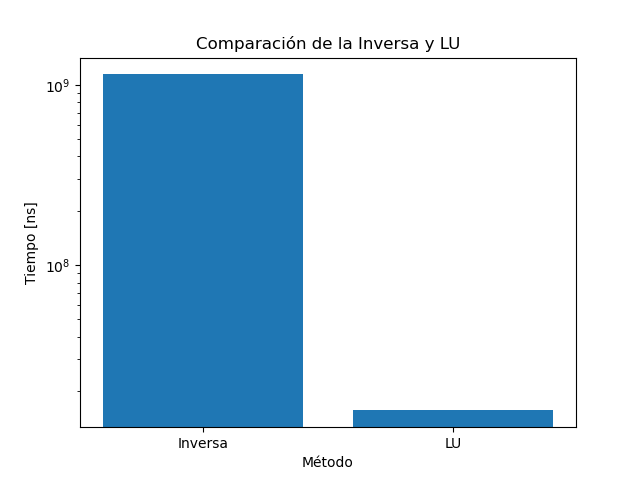
\includegraphics[scale=1]{Figure_1.PNG}
\end{figure}

    
    \hypertarget{conclusiones}{%
\subsection{Conclusiones}\label{conclusiones}}

\begin{itemize}
\tightlist
\item
  Se concluye que el método más eficiente es el de descomposición LU y se puede apreciar que es 73 veces más que el de la inversa.
\item
  Para apreciar un tiempo computacional razonable se debe tener una matriz de dimensiones de 1000 x 1000 debido a la rapidez del cálculo por parte del procesador.
\item
  Se evidencia al realizar varias corridas que el valor de tiempo para la inversa varía, sin embargo, el tiempo computacional para LU se mantiene constante, esto debido a que la matriz es aletaria y en cada corrida es diferente, por tanto para el método de la inversa presenta algunas complicaciones.
\end{itemize}


    % Add a bibliography block to the postdoc
    
    
    
\end{document}
